\documentclass[../main.tex]{subfiles}

\begin{document}

\section{Evaluating discrepancies in hippocampal segmentation protocols using automatic prediction of MRI quality (MRIQC)}

\authors{Jacob Sanz-Robinson\textsuperscript{1}, Mohammad Torabi\textsuperscript{1}, Tyler James Wishard\textsuperscript{2}}

\affiliations{1. Neuroscience, McGill University, Quebec, Canada, 
2. Psychiatry, University of California, Los Angeles, United States}

\subsection{Introduction}

Neuroimaging study results can vary significantly depending on the processing pipelines utilized by researchers to run their analyses, contributing to reproducibility issues. Researchers in the field are often faced with multiple choices of pipelines featuring similar capabilities, which may yield different results when applied to the same data \parencite{carp2012plurality, kennedy2019everything}. While these reproducibility issues are increasingly well-documented in the literature, there is little existing research explaining why this inter-pipeline variability occurs or the factors contributing to it. In this project, we set out to understand what data-related factors impact the discrepancy between popular neuroimaging processing pipelines.

\subsection{Method}

The hippocampus is a structure commonly associated with memory function and dementia, and the left hippocampus is proposed to have higher discriminative power for identifying the progression of Alzheimer’s disease than the right hippocampus in multiple studies \parencite{schuff2009mri}. We obtained left hippocampal volumes using three widely-used neuroimaging pipelines: FSL 5.0.9 \parencite{patenaude2011bayesian}, FreeSurfer 6.0.0 \parencite{fischl2012freesurfer}, and ASHS 2.0.0 PMC‐T1 atlas \parencite{xie2019automated}.
We ran the three pipelines on T1 images from 15 subjects from the Prevent-AD Alzheimer’s dataset \parencite{tremblay2021open}, composed of cognitively healthy participants between the ages of 55-88 years old that are at risk of developing Alzheimer's Disease. 
We ran MRIQC \parencite{esteban2017mriqc} - a tool for performing automatic quality control and extracting quality measures from MRI scans - on the 15 T1 scans and obtained Image Quality Metrics (IQMs) from them. We then found the correlations between the IQMs and the pairwise inter-pipeline discrepancy of the left hippocampal volumes for each T1 scan.

\subsection{Results}

We found that for The FSL-FreeSurfer and FSL-ASHs discrepancies, MRIQC’s EFC measure produced the highest correlation, of 0.69 and 0.64, respectively. The EFC “uses the Shannon entropy of voxel intensities as an indication of ghosting and blurring induced by head motion” \parencite{MRIQCdoc}. No such correlations were found for the ASHS-FreeSurfer discrepancies. \Cref{fig:MRIQC-fig} shows a scatter plot of the discrepancies in left hippocampal volume and EFC IQM for each pipeline pairing. The preliminary results suggest that FSL’s hippocampal segmentation may be sensitive to head motion in T1 scans, leading to larger result discrepancies, but we require larger sample sizes to make meaningful conclusions. The code for our project can be found on GitHub at \href{https://github.com/jacobsanz97/Pipeline-Discrepancy-Exploration}{this link}. 

\begin{figure}
	\centering
	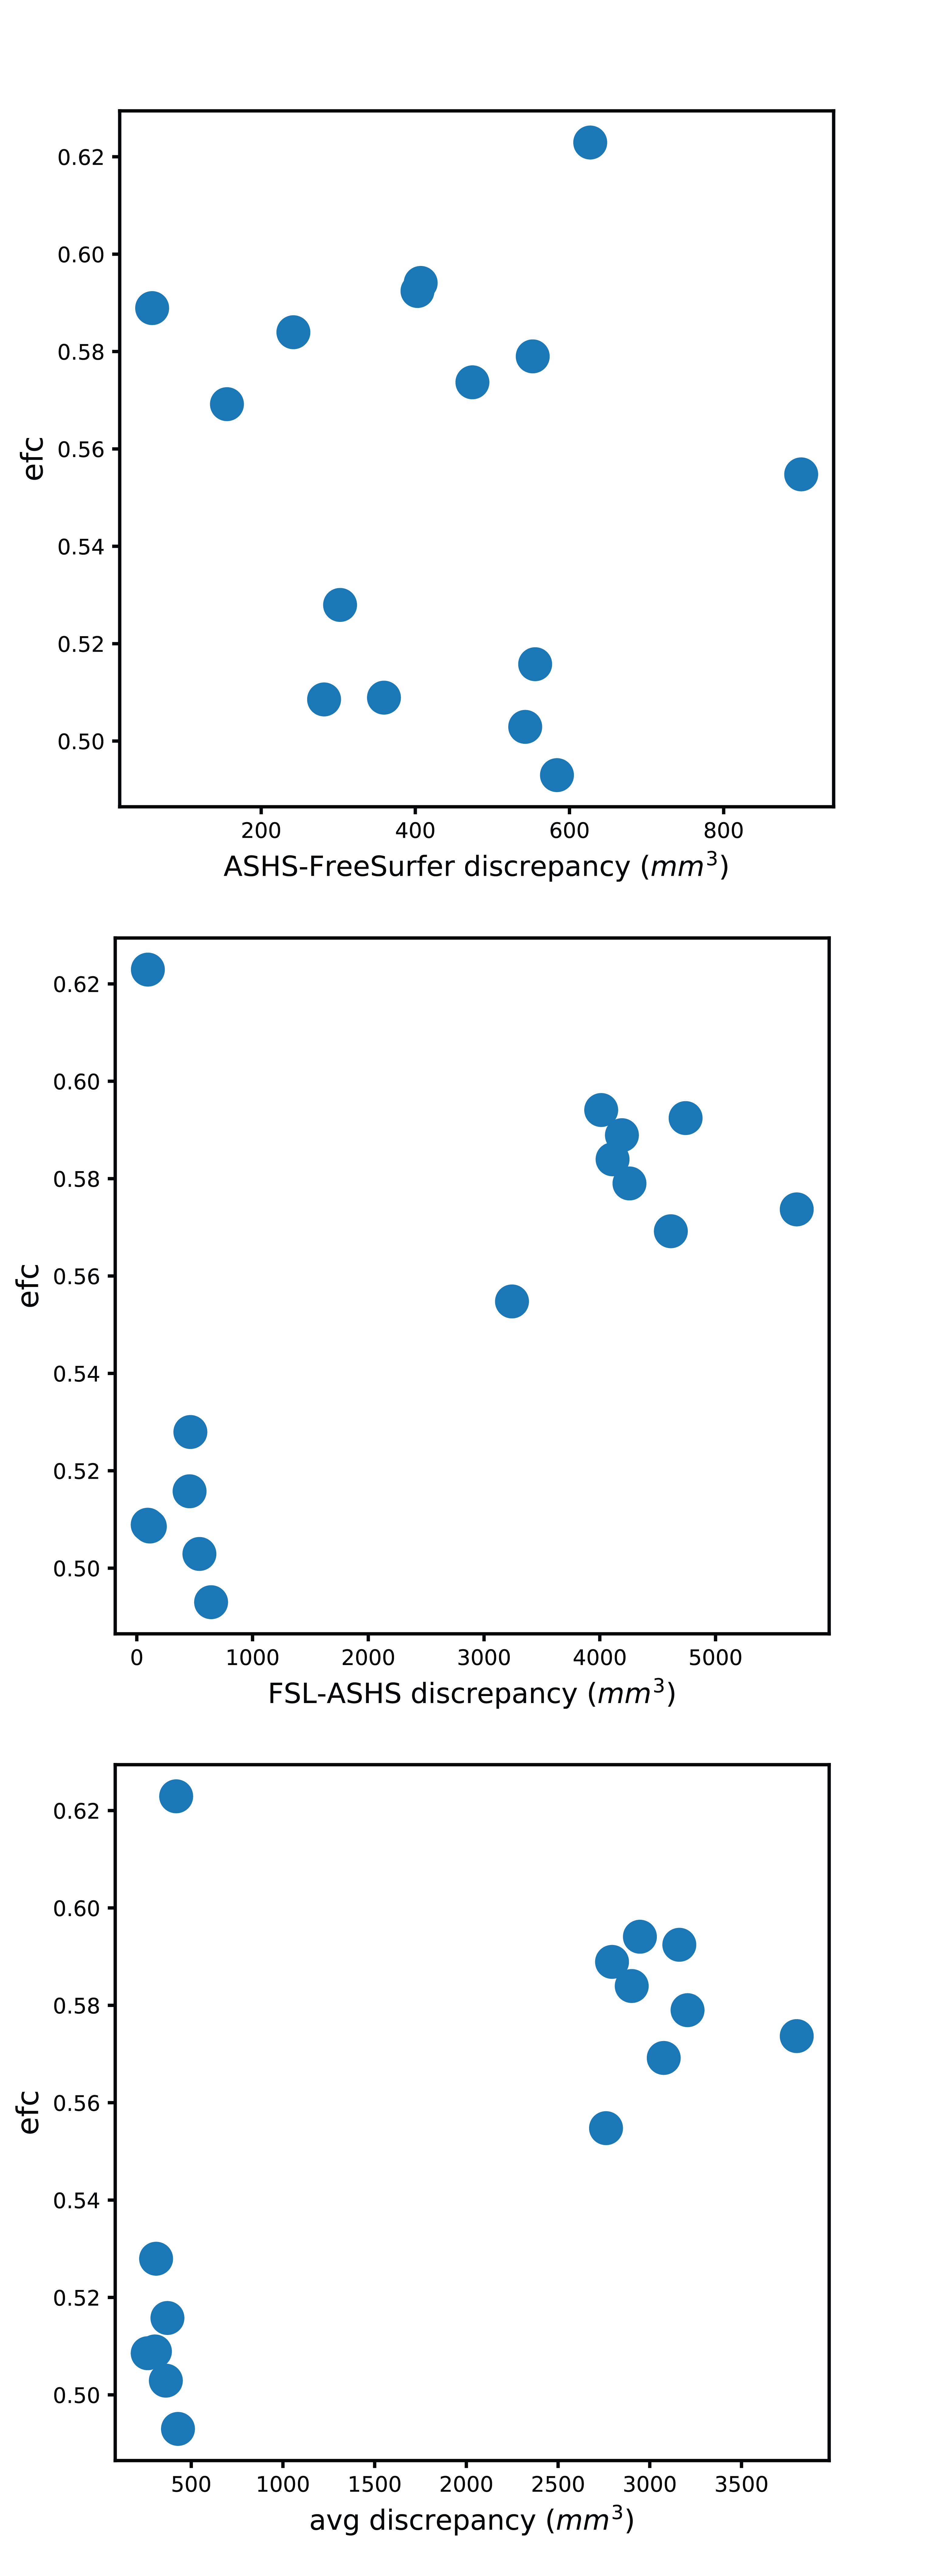
\includegraphics[width=0.4\textwidth]{MRIQC-fig.png}
	\caption{Plots showing the association between left hippocampal volume discrepancies and MRIQC’s EFC quality measure for each of the pipeline pairings.}
	% Add a label to reference in text. Make it specific!
	\label{fig:MRIQC-fig}
\end{figure}

\subsection{Conclusion and Next Steps}

In this project, we investigated the correlation between MRIQC’s IQMs and discrepancies in left hippocampal volume derived from three common neuroimaging pipelines on 15 subjects from the Prevent-AD study dataset. While our preliminary results indicate image ghosting and blurring induced by head motion may play a role in inter-pipeline result discrepancies, the next steps of the project will consist of computing the correlations on the full 308 subjects of the Prevent-AD dataset to investigate whether they persist with the full sample.

\printbibliography

\end{document}
